% Created 2023-12-03 Sun 16:26
% Intended LaTeX compiler: pdflatex
\documentclass[12pt, a4paper]{article}
\usepackage[utf8]{inputenc}
\usepackage[T1]{fontenc}
\usepackage{graphicx}
\usepackage{longtable}
\usepackage{wrapfig}
\usepackage{rotating}
\usepackage[normalem]{ulem}
\usepackage{amsmath}
\usepackage{amssymb}
\usepackage{capt-of}
\usepackage{hyperref}
\usepackage{placeins}
\usepackage{gensymb}
\usepackage[letterpaper]{geometry}
\geometry{top=1.0in, bottom=1.0in, left=1.0in, right=1.0in}
\usepackage{rotating}
\usepackage{graphicx}
\usepackage{pgfplots}
\usepackage{filecontents}
\usepackage{tikz}
\usepackage{fancyhdr}
\usepackage{enumitem}
\pagestyle{fancy}
\lhead{}
\chead{}
\rhead{Johnson \thepage}
\lfoot{}
\cfoot{}
\rfoot{}
\renewcommand{\headrulewidth}{0pt}
\renewcommand{\footrulewidth}{0pt}
\setlength\headsep{0.333in}
\newcommand{\bibent}{\noindent \hangindent 40pt}
\newenvironment{workscited}{\newpage \begin{center} Works Cited \end{center}}{\newpage }
\graphicspath{ {./attachments/} }
\author{Christian}
\date{\today}
\title{}
\hypersetup{
 pdfauthor={Christian},
 pdftitle={},
 pdfkeywords={},
 pdfsubject={},
 pdfcreator={Emacs 28.2.50 (Org mode 9.7-pre)}, 
 pdflang={English}}
\begin{document}

\begin{document}
\begin{flushleft}
Christian Johnson\\
\vspace{2mm}Dr. Paul Crilly\\
\vspace{2mm}Antennas and Propogation\\
\vspace{2mm}December 03 2023\\
\vspace{4mm}\begin{center}
Lab 8 Report
\end{center}
\vspace{1mm}\setlength{\parindent}{0.5in}
\begin{abstract}
This lab concentrated on the comprehensive process of designing, simulating, constructing, and testing a Yagi antenna. Employing MATLAB for design and optimization, the antennas were physically constructed using PVC piping and copper rods. However, challenges in optimizing the simulation forced the use of default measurements from the antenna handbook. Consequently, the radiation pattern may not have been fully optimized for directionality, though the antenna remained functional. During the testing phase with the Agilent FieldFox and a transmitter,

[observations indicated the effectiveness of the antenna in transmitting and receiving signals. However, detailed results comparing the actual radiation pattern to the expected pattern need further analysis].

\end{abstract}
\section*{Procedures}
\label{sec:org5cb3720}
This lab was broken into three seperate parts, simulation, construction, and testing.
The simulation section focused on using MATLAB to simulate and optimize the antennas radiation pattern, given default measurements provided in the ARRL Antenna Book for a frequency of 145 MHz. The eventual goal was to maximize the front to rear ratio and front to side ratio of the antenna's radiation pattern.
The next section focused on constructing the actual antenna using the given materials. The primary components used for this antenna were 3/4" PVC pipe, 1/8" welding rod, PVC T connections, BNC connectors, and metal screws. Using the measurements obtained from the simulation, 1/8" holes were drilled into the PVC to hold the copper elements. Once the elements were trimmed to length, they were inserted into these holes and secured with screws. The driven element was formed from a bent wire, forming a loop that connected back to a BNC connector in order to allow Coaxial connections. Finally, the antenna was divided in half and connected using a T connector, with a longer piece of piping extending below to serve as a handle. 
The final section of this lab involved testing the radiation pattern for the antenna. Using an Agilent 9912A Field Fox Analyzer in linear mode, it was configured to receive the signal emanated by another, seperate Field Fox connected as a signal source. With one group member holding the antenna, and another reading the analyzer, the antenna was rotated in a complete circle, stoppingto take measurements every 45 degrees. These measurements are used to compare to the graphs in the simulations taken during section 1 of this lab. 
\section*{Results}
\label{sec:org222ba5b}

We initially faced difficulty optimizing our radiation pattern in MATLAB. After several failed iterations, we eventually opted to use the default measurements provided in the ARRL Antennas Handbook. These values specified 2 directors, with lengths in meters of 0.9525 and 0.8382 and spacing in meters of 0.1997 and 1.2887. The reflector had length 1.0514m and spacing 0.0000001m, and the exciter (or driven element) with length of 0.9979m, width of 0.0254m, and spacing of 0.001m. In the simulation program, these results produce a nearly circular radiation pattern, with a large front to side ratio, and a one to one front to back ration.
We were able to effectively construct our antenna, although we were forced to replace our BNC connector after melting it the first time. After construction, we began testing our antenna. Measuring our antennas SWR at different azimuths in intervals of 45 degrees, we obtained values described in the following table.
\begin{center}
\begin{tabular}{rl}
SWR & Azimuth\\[0pt]
-68 & 0 degrees\\[0pt]
-73 & 45 degrees\\[0pt]
-76.5 & 90 degrees\\[0pt]
-83.5 & 135 degrees\\[0pt]
-82.5 & 180 degrees\\[0pt]
-77 & 225 degrees\\[0pt]
-87.5 & 270 degrees\\[0pt]
-71 & 315 degrees\\[0pt]
\end{tabular}
\end{center}

\begin{figure}[htb]
\centering
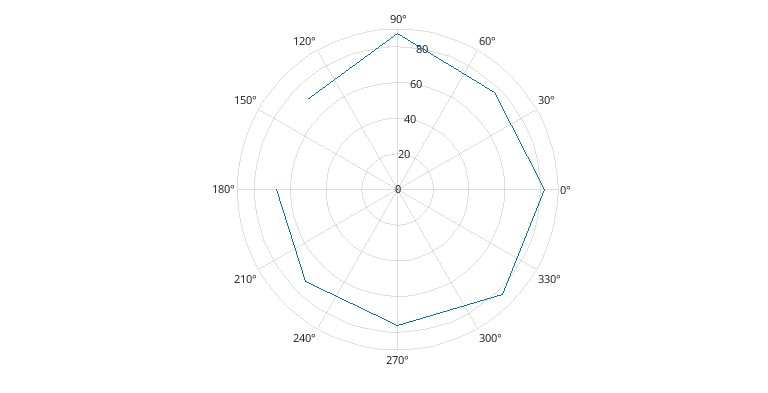
\includegraphics[width=0.7\textwidth]{Polarplot.jpg}
\caption{Polar Plot of SWR measurements}
\end{figure}

This graph shows a circle, with relatively consistant SWR values across the entire range of angles. This indicates that our antenna was poorly designed, and was not directional enough to make a noticeable difference. Perhaps if we had taken measurements at smaller increments we might have seen a better response, but this imperfection likely stems from our failure to properly optimize our radiation pattern in the first part of this lab.
In the end, given the number of measurements we took, it seems that our data lines up with the radiation pattern produced from the simulation. 
\section*{Conclusions}
\label{sec:org8636b5b}

The Yagi antenna lab provided a comprehensive exploration of the design, construction, and testing processes. Initially challenged with optimizing the radiation pattern using MATLAB, we turned to default measurements from the ARRL Antennas Handbook. These specifications, involving 2 directors, a reflector, and an exciter, formed the basis for our physical antenna.

The construction phase revealed practical challenges, including the need to replace a melted BNC connector. Despite this setback, the assembly adhered to the simulation-derived dimensions. Testing the antenna's SWR at different azimuths produced results indicative of its performance. The obtained polar plot, displaying a nearly circular pattern with consistent SWR values, suggested a less-than-optimal design, possibly attributable to our initial simulation difficulties.

While our antenna demonstrated functionality, the lack of noticeable directionality highlights the critical importance of accurately optimizing the radiation pattern during the simulation phase. The imperfections observed in the polar plot underscore the need for precision in antenna design.

In retrospect, taking measurements at smaller increments during testing might have provided a more detailed understanding of the antenna's behavior. Nevertheless, our data aligns with the radiation pattern produced from the simulation, emphasizing the impact of simulation accuracy on the final antenna performance.

This lab reinforces the significance of meticulous simulation and design processes in achieving optimal antenna characteristics. Future iterations could benefit from improved simulation techniques and a more thorough understanding of the relationship between design parameters and real-world performance.

\newpage
\begin{center}
Appendices
\end{center}
\begin{figure}[htb]
\centering
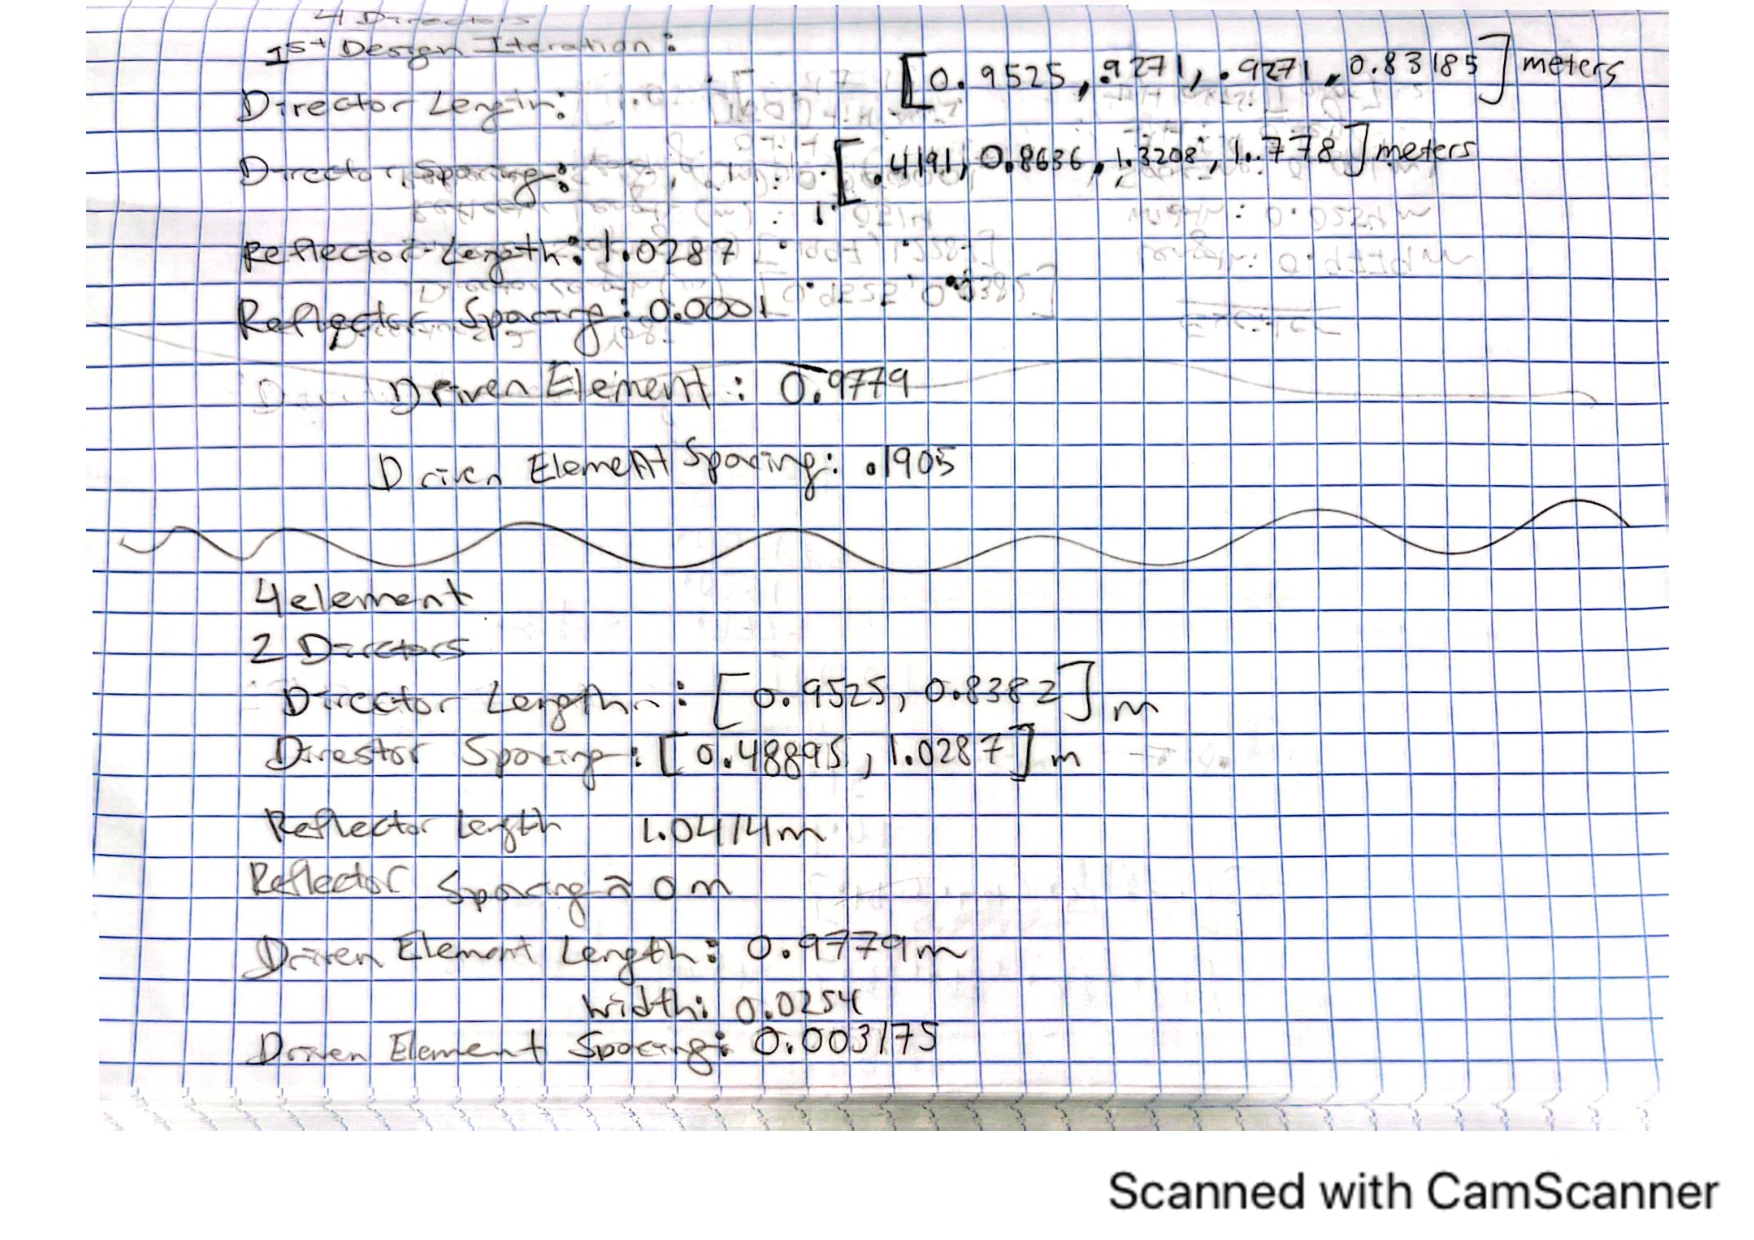
\includegraphics[page=1,width=0.4\textwidth]{LabNotebook.pdf}
\caption{Notebook Page 1}
\end{figure}
\begin{figure}[htb]
\centering
\includegraphics[page=2,width=0.4\textwidth]{LabNotebook.pdf}
\caption{Notebook Page 2}
\end{figure}
\newpage
\begin{figure}[htb]
\centering
\includegraphics[page=3,width=0.4\textwidth]{LabNotebook.pdf}
\caption{Notebook Page 3}
\end{figure}
\begin{figure}[htb]
\centering
\includegraphics[page=4,width=0.4\textwidth]{LabNotebook.pdf}
\caption{Notebook Page 4}
\end{figure}
\newpage
\newpage
\newpage

\begin{center}
Lab Questions
\end{center}
\vspace{2mm}
\begin{enumerate}[label=\textbf{\arabic*.}]
\item To what degree does the polar plot look like the simulations?
The polar plot looks nearly circular, with relatively consistant SWR values. This differs from the simulation expectations, which anticipated a more directional radiation pattern. The deviation can be attributed to the challenges faced in optimizing the radiation pattern during the simulation phase.
\item Why does the optimum SWR occur at other than 1/2 wavelength of the driven element?
This could be influenced by factors like Antenna loading (the presence of additional elements like directors or reflectors that can alter the electrical length), Matching Networks, or Antenna Configuration (the specific configuration can influence the resonance point).
\item Other designs considered.
We chose our final design based on necessity, since we could not get anything else to work. We attempted to adjust several values in the simulation software, but most values gave us lopsided, nondirectional radiation patters. As imperfect as our final antenna ended up being, the default configuration was still the best we achieved in our simulations.
\item What is the front to back and front to side ratio?
The front to back and front to side ratios in our data are both close to 1. In the simulations, front to back was also 1, so this matches well, but our simulations also gave us a front to side ratio close to 3 or 4, which our data does not show. I suspect that performing a test with more data points might reveal a higher front to side ratio, since the notch in the simulation was rather small.
\item What is the 3dB beamwidth?
In our data, we never seem to drop to 1/2 of the maximum SWR (which is where we would find the 3dB beamwidth).
\item What is the approximate length for the driven element of a yagi operating at a) 7MHz b) 14MHz and c) 1GHz
a) 21.43m b) 10.72m c) 0.15m
\item Why is a yagi impractical for frequencies above 1GHz?
The element sizes become impractically small, making construction challenging. Alternate designs are more practical and more efficient, making yagi antennas ill suited for these frequencies.
\item What are at least 2 significant advantages of using  a T-match + BALUN instead of a gamma match?
Balanced transmission: The T Match with a balun helps to achieve balanced transmission, reducing current and minimizing unwanted radiation. Versatility: T match with a balun can provide a broader range of impedance matching possibilities, making it adaptable to various antenna designs and configurations.
\end{enumerate}

\end{document}
\end{document}